\section{Image as Functions}
\label{sec:image_as_functions}

\subsection{A Brief History}

\subsection{Image as Functions}
图片定义成一个函数 $f: \R^2 \to \R^M$ ,其中 $M$ 是颜色通道的数量,通常是 1 (灰度图) 或 3 (RGB 图). 
\begin{itemize}
    \item \textbf{Pixel value}: intensity in $[0, 255]$ and color with 3 channels $[R, G, B]$.
    \item \textbf{Resolution}: $H \times W$. 
    \item An image contains discrete number of pixels $\to$ A tensor with $[H, W, C]$.
\end{itemize}

\subsection{Image Gradient}
Image $f(x, y)$ $\implies$ Gradient $\nabla f(x, y) = \left[ \frac{\partial f}{\partial x}, \frac{\partial f}{\partial y} \right]$.

在实际中是一个有限差分的近似:
\begin{equation}
    \frac{\partial f}{\partial x} \bigg|_{(x, y)=(x_0, y_0)} \approx \frac{f(x_0 + 1, y_0) - f(x_0 - 1, y_0)}{2}
\end{equation}

对于图片我们将梯度可视化可以得到 Gradient Maginitude, 间接反映图片的纹理和边缘信息.
\[
    \text{Gradient Magnitude} = \norm{\nabla f} = \sqrt{\left( \frac{\partial f}{\partial x} \right)^2 + \left( \frac{\partial f}{\partial y} \right)^2}
\]
% TODO: Add a figure to illustrate the gradient magnitude.

\subsection{(Signal) Convolution Filter}
\subsubsection{Quick Facts of Convolution}
下图展示了离散信号和连续信号的卷积操作:
\[
\begin{array}{ccc}
    \hline
    & \text{Discrete Signal} & \text{Continuous Signal} \\
    \hline
    \text{Convolution} & (f * g)[n] = \sum_{i = -\infty}^{\infty} f[i] g[n - i] & (f * g)(t) = \int_{-\infty}^{\infty} f(\tau) g(t - \tau) d\tau \\
    \text{Fourier Transform} & \mathcal{F}[n] = \sum_{m = 0}^{M-1} f[m] \exp\left( -\frac{2\pi i}{M} m n \right) & \mathcal{F}(f) = \int_{-\infty}^{\infty} f(t) \exp(-2\pi i \omega t) dt \\ 
    \hline
\end{array}
\]

对于卷积操作最重要的性质是 \textbf{Convolution Theorem}, 它告诉我们在时域上的卷积等价于频域上的乘积\marginpar{\kaishu Fourier变换将时域信号转化为频域信号}, 即:
\[
    \mathcal{F}(f * g) = \mathcal{F}(f) \cdot \mathcal{F}(g) \implies f * g = \mathcal{F}^{-1}(\mathcal{F}(f) \cdot \mathcal{F}(g))
\]

这个定理使得我们可以使用傅立叶变换与逆变换来便捷的计算卷积操作. 此外, 对于卷积的微分有如下性质
\[
    \frac{\dd }{\dd x} (f * g) = f * \frac{\dd }{\dd x} g
\]

按照傅立叶变换后的滤波函数的集中情况, 可以将滤波器分为:
\begin{itemize}
    \item 低通滤波器(Low-pass Filter) 滤去高频信号, 保留低频信号. 
    \item 高通滤波器(High-pass Filter) 滤去低频信号, 保留高频信号.
    \item 带通滤波器(Band-pass Filter) 只保留某个频率段的信号.
    \item 带阻滤波器(Band-stop Filter) 只滤去某个频率段的信号.
\end{itemize}
\begin{figure}[htbp]
    \centering
    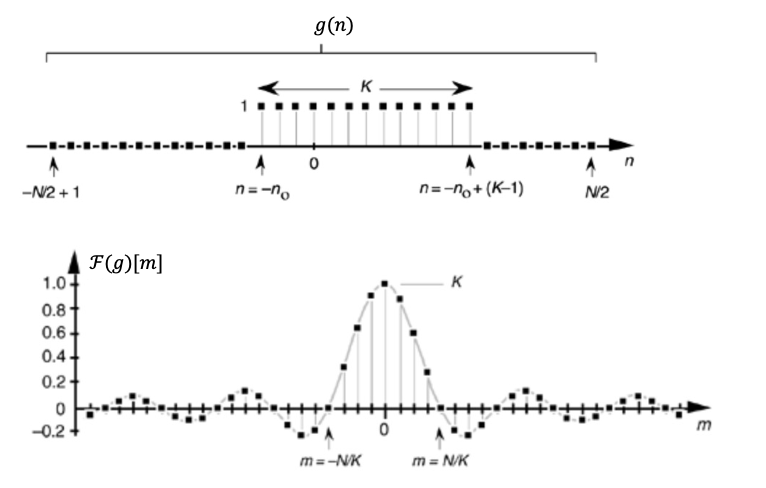
\includegraphics[scale=0.75]{figures/Fourier.png}
    \caption{Rectangular Function and its Fourier Transform(A low-pass filter)}
\end{figure}


\subsubsection{1D Discrete-Space Filter} 
在一维上信号 $f[n]$ 经过系统 $\mathcal{G}$ 后得到输出 $h[n]$, 可以表示为:
\[
    f[n] \to \fbox{\text{System } $\mathcal{G}$} \to h[n], \quad \text{Output: } h[h] = \mathcal{G}(f)[n]
\]

例如 Moving Average Filter, 在局部区域内取平均值 (假设前后的噪声是独立的, 通过平均值可以使得噪声相互抵消.)
\[
    h[n] = \frac{1}{k} \sum_{i = n}^{n + k} f[i]
\]

能够抑制高斯噪声, 但是会使得信号的边缘变得平滑(直接跳迁变为渐变). 更一般的可以定义为卷积(Convolution)操作:
\[
    h[n] = (f * g)[n] = \sum_{i = -\infty}^{\infty} f[i] g[n - i]
\] 

其中 $g[n]$ 是卷积核, 也叫做滤波器(Filter). \marginpar{\kaishu Move Average Filter 是一种低通滤波器, 可以滤去高频噪声, 而保留低频原始信号.}

如何解决信号的边缘平滑问题? $\implies$ 设计更好的滤波器. $\implies$ 在深度学习中, 通过 Learning 得到更好的滤波器/卷积核.

\subsubsection{2D Discrete-Space Filter}
对于二维信号 $f(x, y)$, 这里简单列出卷积操作的定义:
\begin{equation*}
    f[n, m] \to \fbox{\text{System } $\mathcal{G}$} \to h[n, m], \quad \text{Output: } h[h, m] = \mathcal{G}(f)[n, m]
\end{equation*}
\begin{equation*}
    h[n, m] = (f * g)[n, m] = \sum_{k, l} f[k, l] g[n - k, m - l]
\end{equation*}

使用一个全1的卷积核(即二维下的 Moving Average Filter)可以得到一个平滑的图像, 但是会使得图像的边缘变得模糊. \marginpar{\kaishu 边缘附近像素会发生跳变, 是高频信号}

这里我们可以使用 Binarization via Thresholding (阈值二值化, Non-linear Filter) 来处理上述边缘模糊问题. 即设置阈值 $\tau$, 将大于 $\tau$ 的像素设为 1, 小于 $\tau$ 的像素设为 0.
\[
    h[n, m] = \begin{cases}
        1, & \text{if } f[n, m] > \tau \\
        0, & \text{otherwise}
    \end{cases}
\]
\marginpar{\kaishu 图为燕园的猫雪风}
\begin{figure}[htbp]
    \centering
    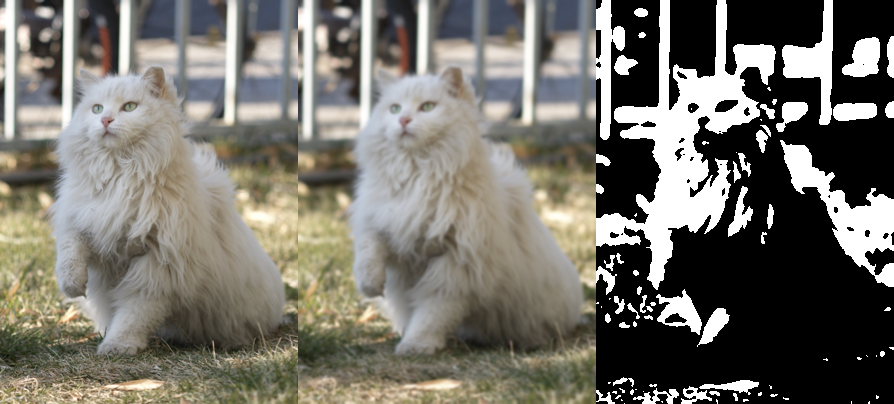
\includegraphics[scale=0.35]{figures/cat_gaussian.png}
    \caption{Visualizing the effect of Gaussian Filter and Binarization}
\end{figure}

